\documentclass{beamer}
\usetheme{metropolis}
\usepackage{booktabs}
\usepackage{pgfplots}
\usepackage{pax}
\usepackage{caption}
\usepgfplotslibrary{dateplot}
\renewcommand{\tablename}{\textbf{Taula}}
\renewcommand{\figurename}{\textbf{Figura}}

\title{TREBALL FINAL DE GRAU}

\subtitle{Disseny d'una eina per al tractament i visualització de les dades d'accés a un repositori}
\date{10 Juliol, 2024}
\author{Omar Briqa}
\institute{Escola Politècnica Superior d'Enginyeria de Vilanova i la Geltrú}

\begin{document}

\maketitle
\begin{frame}{Sumari}
    \setbeamertemplate{section in toc}[sections numbered]
    \tableofcontents
\end{frame}

\section{Introducció}\label{sec:introduction}
\section{Processament de les dades}\label{sec:data-processing}

\begin{frame}{Registres d'accés}

\begin{figure}
    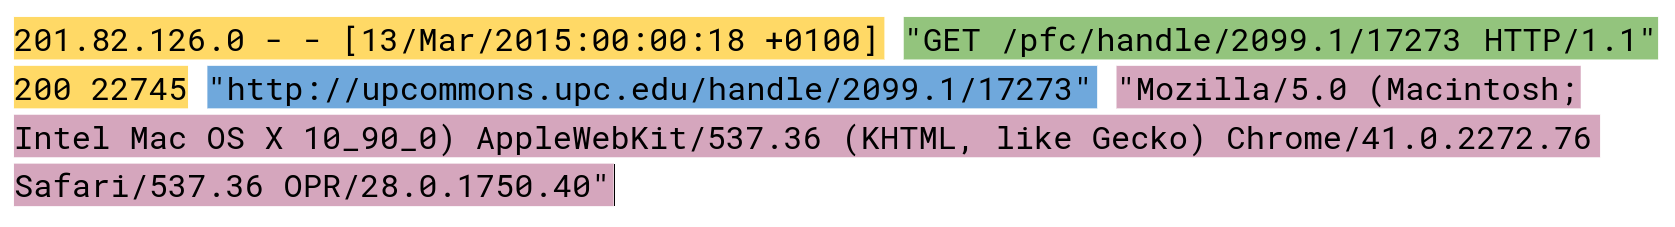
\includegraphics[width=\textwidth]{figures/example-log}
    \label{fig:log-example}
\end{figure}

\begin{itemize}%[<+- | alert@+>]
    \item Informació de la petició HTTP.
    \begin{itemize}%[<+- | alert@+>]
        \item Adreça IP: informació \textbf{personal}, s'ha hagut de passar per un procés d'anonimització.
        \item Data i hora
        \item Informació de la petició HTTP
        \item Referent
        \item User Agent
    \end{itemize}
\end{itemize}

\end{frame}

\begin{frame}{Filtratge dels \textit{logs} I}
    \begin{itemize}%[<+- | alert@+>]
        \item Durant el processament hem trobat diverses casuístiques que s'han de tractar detalladament.
        \begin{itemize}%[<+- | alert@+>]
            \item Accés a recursos web.
            \item Repeticions.
            \item Cerques.
            \item Errors de processament.
            \begin{itemize}%[<+- | alert@+>]
                \item Errors reversibles.
                \item Errors irreversibles.
            \end{itemize}
        \end{itemize}
    \end{itemize}
\end{frame}

\begin{frame}{Accés a recursos web}
    \begin{itemize}%[<+- | alert@+>]
        \item Aquests casos els descartem.
    \end{itemize}

    \begin{figure}[htbp]
        \centerline{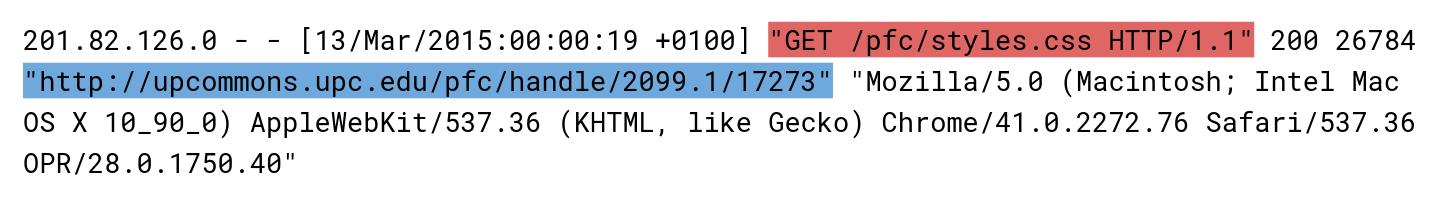
\includegraphics[width=\textwidth]{figures/log-web-resource}}
        \label{fig:log-web-resource}
    \end{figure}
\end{frame}

\begin{frame}{Repeticions}
    \begin{itemize}%[<+- | alert@+>]
        \item Accessos ``repetits'' al mateix recurs.
    \end{itemize}
    \begin{figure}[htbp]
        \centerline{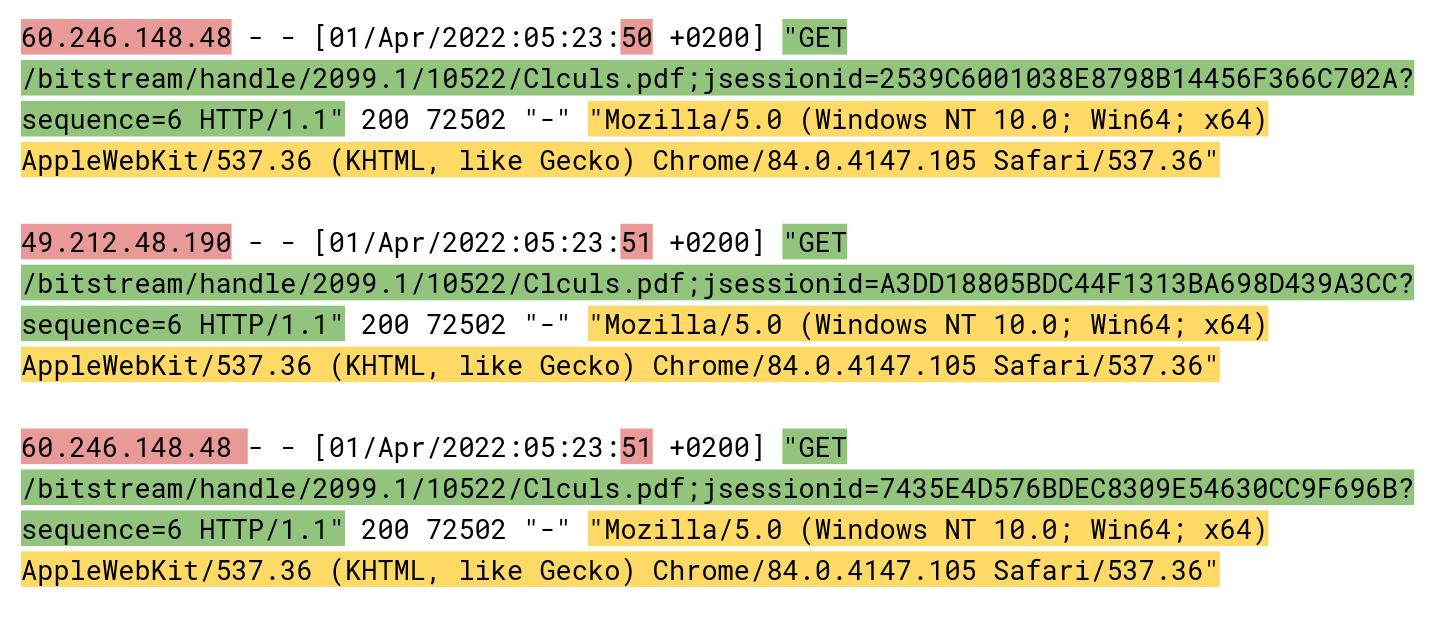
\includegraphics[width=\textwidth]{figures/log-repetitions}}
        \label{fig:log-repetitions}
    \end{figure}
\end{frame}

\begin{frame}{Cerques}
    \begin{itemize}%[<+- | alert@+>]
        \item Aquests casos els marquem com a cerques.
    \end{itemize}
    \begin{figure}[htbp]
        \centerline{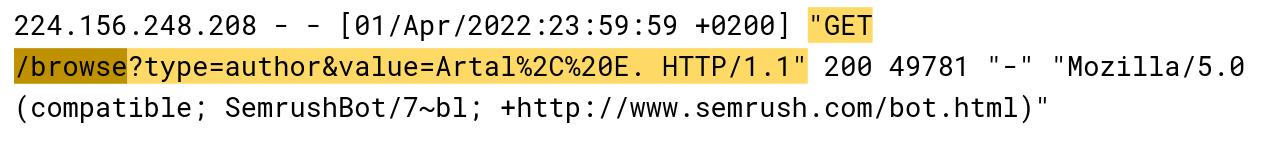
\includegraphics[width=\textwidth]{figures/log-search}}
        \label{fig:log-search}
    \end{figure}
\end{frame}

\begin{frame}{Errors de processament}
    \begin{itemize}%[<+- | alert@+>]
        \item Aquells que segueixin un paradigma, manipularem el registre afectat per homogeneïtzar el conjunt dels logs.
        \item Els errors que no hem pogut adaptar-los s'han descartat.
    \end{itemize}
    \begin{figure}[htbp]
        \centerline{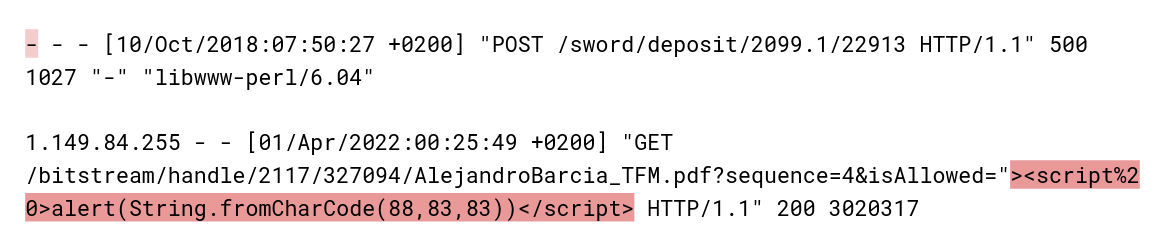
\includegraphics[width=\textwidth]{figures/log-error}}
        \label{fig:log-error}
    \end{figure}
\end{frame}

\begin{frame}{Disseny del processament dels logs}

    \begin{figure}
        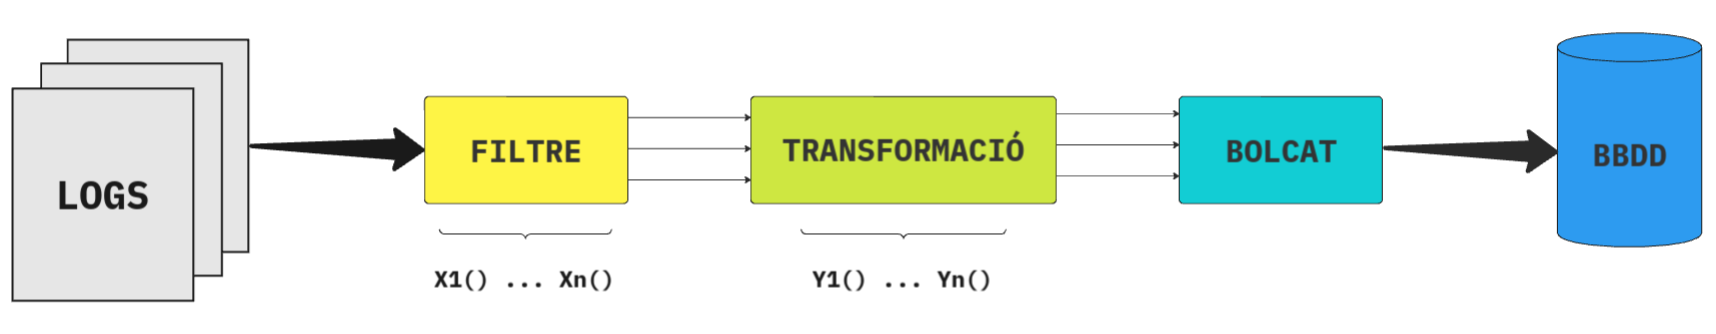
\includegraphics[width=\textwidth]{figures/log-processing}
        \label{fig:log-processing}
    \end{figure}

    \begin{itemize}%[<+- | alert@+>]
        \item Tres components.
        \begin{itemize}%[<+- | alert@+>]
            \item \texttt{Filtre} \(\rightarrow\) Filtra cada \textit{log} mitjançant un criteri específic.
            \item \texttt{Transformació} \(\rightarrow\) Modifica el format del \textit{log} per afegir o treure camps.
            \item \texttt{Bolcat} \(\rightarrow\) Adapta el format i envia el \textit{log} a la base de dades.
        \end{itemize}
    \end{itemize}
\end{frame}


\begin{frame}{Implementació del processament}
    \begin{figure}
        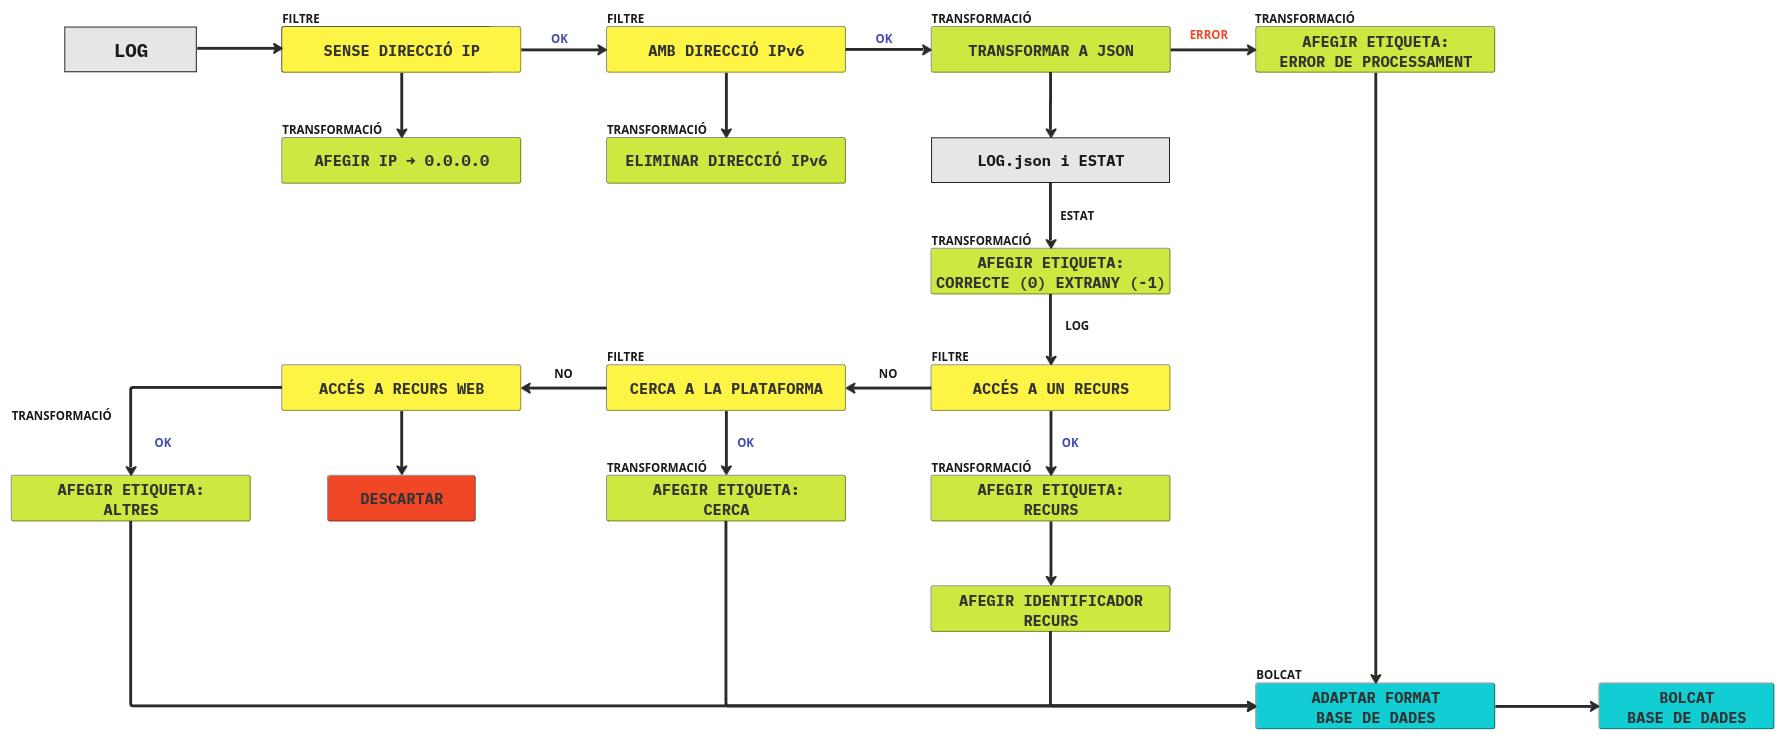
\includegraphics[width=1\textwidth]{figures/log-processing-workflow}
        \label{fig:log-processing-workflow}
    \end{figure}
\end{frame}


\begin{frame}{Metadades}
    \begin{itemize}%[<+- | alert@+>]
        \item Conjunt d’etiquetes presents als recursos d’UPCommons que contenen informació sobre aquest.
        \item Format: DSpace Intermediate Metadata (DIM):
        \begin{itemize}%[<+- | alert@+>]
            \item Dublin Core + qualificador.
        \end{itemize}
        \item Exemple: autor principal d'un recurs.
        \begin{itemize}%[<+- | alert@+>]
            \item \texttt{schema.element.qualifier} \(\rightarrow\) \texttt{dc.contributor.author}
        \end{itemize}
    \end{itemize}
\end{frame}


\begin{frame}{Descàrrega de les metadades}

    \begin{figure}
        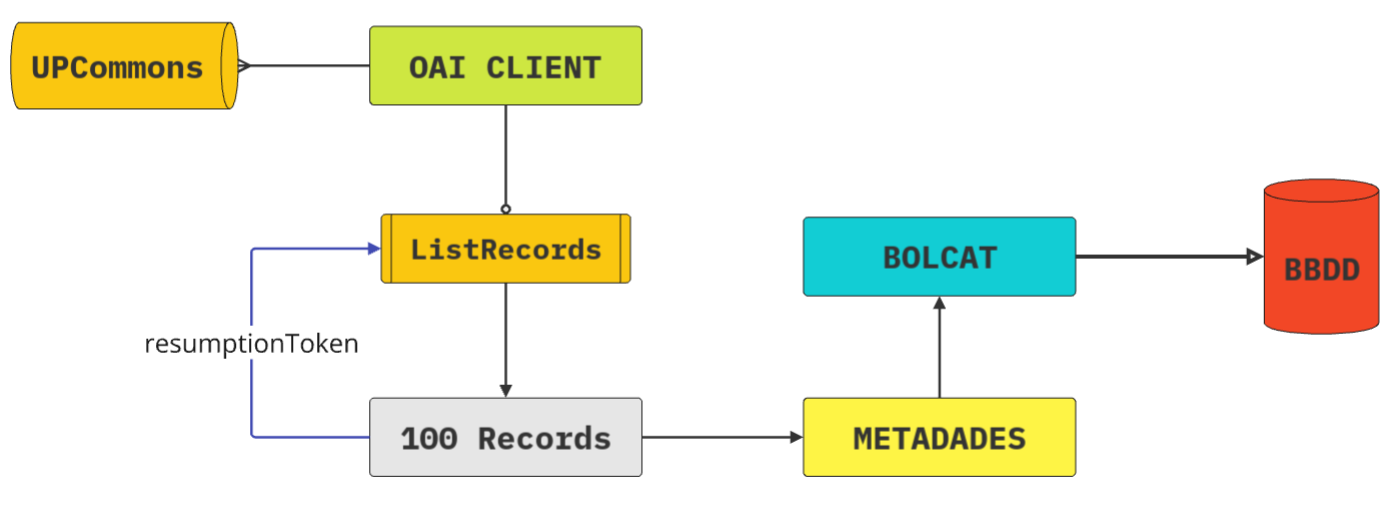
\includegraphics[width=\textwidth]{figures/metadata-processing}
        \label{fig:metadata-processing}
    \end{figure}

    \begin{itemize}%[<+- | alert@+>]
        \item Utilitzarem el protocol OAI-PMH (Open Archive Initiative-Protocol for Metadata Harvesting).
        \item El servidor que emmagtzema aquestes metadades implementa un mecansime de control de flux basat en el \textit{resumptionToken}.
    \end{itemize}

\end{frame}
\section{Emmagatzematge de les dades}\label{sec:data-storing}

\begin{frame}{Format dels \textit{logs}}

    \begin{itemize}
        \item Aquests són els camps principals d'interés que obtenim directament dels \textit{logs}.
        \item El pas dels anys (i el canvi de les versions de DSpace) no han fet que canviï gaire el format.
        \begin{itemize}
            \item \texttt{ip\_address}
            \item \texttt{time}
            \item \texttt{request}
            \begin{itemize}
                \item \texttt{method}
                \item \texttt{resource}
                \item \texttt{version}
                \item \texttt{status\_code}
                \item \texttt{response\_size}
            \end{itemize}
            \item \texttt{referer}
            \item \texttt{user\_agent}
        \end{itemize}
    \end {itemize}
\end{frame}


\begin{frame}{Base de dades pels logs}
    \begin{itemize}%[<+- | alert@+>]
        \item Característiques:
        \begin{itemize}
            \item Base de dades de codi obert.
            \item Enfocada a registres d'accés.
            \item Ben documentada, actualitzada i mantinguda per una comunitat activa d'usuaris.
            \item Capacitat per processar grans quantitats de dades.
            \item Capacitat d'allotjar la nostra base de dades localment al nostre servidor de treball.
        \end{itemize}
        \item Hem considerat diverser opcions: Loki, Elastic, SOLR, InfluxDB, etc.
        \item Decisió final: InfluxDB.
    \end{itemize}
\end{frame}


\begin{frame}{Paràmetres adicionals d'InfluxDB}
    \begin{itemize}%[<+- | alert@+>]
        \item \texttt{tag set}: conjunt de parelles clau-valor \textbf{indexades}.
        \begin{itemize}
            \item \textbf{content}: format del contingut, pot ser:
            \begin{itemize}
                \item \texttt{ok}: el format del \textit{log} és l'esperat.
                \item \texttt{diferent}: el format del \textit{log} no és l'esperat, però s'ha pogut tractar.
                \item \texttt{error}: error de processament.
            \end{itemize}
            \item \textbf{method}: mètode HTTP present al \textit{log}.
            \item \textbf{status\_code}: codi d'estat de la resposta de la petició d'HTTP.
            \item \textbf{type}: tipus de \textit{log}, pot ser:
            \begin{itemize}
                \item \texttt{cerca}: cerca a la plataforma d'UPCommons.
                \item \texttt{recurs}: accés a un recurs d'UPCommons.
                \item \texttt{altres}: altres tipus de \textit{log}.
            \end{itemize}
        \end{itemize}
        \item \texttt{field set}: conjunt de parelles clau-valor \textbf{no indexades}.
        \begin{itemize}
            \item \textbf{log}: registre complet d'UPCommons.
            \item \textbf{recurs}: identificador handle, en cas que es tracti d'un accés a un recurs.
        \end{itemize}
    \end{itemize}
\end{frame}


\begin{frame}{Resultat de l'abocament dels logs I}
    \begin{table}[!t]
        \label{tab:table1}
        \centering
        \begin{tabular}{@{} lr @{}}
            \toprule
            \textbf{2006-2023} & Total\\
            \midrule
            Nº total de \textit{logs}       & 1.922.392.760\\
            Accés a recursos UPCommons      & 1.208.133.268\\
            Cerques a UPCommons             & 179.937.769\\
            Accés a recursos web descartats & 430.789.238\\
            Altres tipus de \textit{logs}   & 107.198.724\\
            Errors de processament          & 552\\
            Duració (minuts)                & 1.977,13\\
            \bottomrule
        \end{tabular}
    \end{table}
\end{frame}

\begin{frame}{Resultat de l'abocament dels logs II}

    \begin{figure}
        \begin{tikzpicture}
            \begin{axis}[
                mlineplot,
                width=\textwidth,
                height=0.7\textheight,
                ylabel=Logs,
                xtick={2006, 2008, 2010, 2012, 2014, 2016, 2018, 2020, 2022},
                xticklabel style={/pgf/number format/1000 sep=},
                yticklabel style={/pgf/number format/fixed,/pgf/number format/precision=1},
                legend style={at={(0.5,-0.2)}, anchor=north, legend columns=2, /tikz/every even column/.append style={column sep=0.5cm}}
            ]
                \addplot coordinates {
                    (2006, 1553768)
                    (2007, 14970518)
                    (2008, 30747039)
                    (2009, 37399831)
                    (2010, 76099876)
                    (2011, 109822586)
                    (2012, 109646515)
                    (2013, 70230167)
                    (2014, 68059608)
                    (2015, 146599579)
                    (2016, 139559925)
                    (2017, 133645398)
                    (2018, 140353396)
                    (2019, 127218126)
                    (2020, 166038130)
                    (2021, 192986484)
                    (2022, 189863676)
                    (2023, 167515925)
                };
                \addlegendentry{Nº total de \textit{logs}}
                \addplot coordinates {
                    (2006, 239410)
                    (2007, 3039294)
                    (2008, 8563620)
                    (2009, 17399497)
                    (2010, 44754685)
                    (2011, 78153547)
                    (2012, 80527672)
                    (2013, 33835954)
                    (2014, 28482567)
                    (2015, 97702657)
                    (2016, 95919593)
                    (2017, 80272838)
                    (2018, 90823546)
                    (2019, 83529395)
                    (2020, 99891136)
                    (2021, 124302571)
                    (2022, 126879940)
                    (2023, 113815346)
                };
                \addlegendentry{Recursos d'UPCommons}
                \addplot coordinates {
                    (2006, 584614)
                    (2007, 2043778)
                    (2008, 7421858)
                    (2009, 3987884)
                    (2010, 12385336)
                    (2011, 12493351)
                    (2012, 11728372)
                    (2013, 16093356)
                    (2014, 14118753)
                    (2015, 16117702)
                    (2016, 11252974)
                    (2017, 14075887)
                    (2018, 12055214)
                    (2019, 6815726)
                    (2020, 11351531)
                    (2021, 10237352)
                    (2022, 10820565)
                    (2023, 6353516)
                };
                \addlegendentry{Cerques a UPCommons}
                \addplot coordinates {
                    (2006, 325932)
                    (2007, 7997613)
                    (2008, 10402957)
                    (2009, 11133194)
                    (2010, 9946743)
                    (2011, 11428684)
                    (2012, 13582288)
                    (2013, 17432325)
                    (2014, 21320545)
                    (2015, 24590560)
                    (2016, 24606115)
                    (2017, 28598003)
                    (2018, 32576258)
                    (2019, 32556241)
                    (2020, 48773842)
                    (2021, 51119990)
                    (2022, 48192917)
                    (2023, 36205031)
                };
                \addlegendentry{Recursos web descartats}
            \end{axis}
        \end{tikzpicture}\label{fig:log-push-results}
    \end{figure}

\end{frame}


\begin{frame}{Resultat de l'abocament dels logs III}

    \begin{figure}
        \begin{tikzpicture}
            \begin{axis}[
                mlineplot,
                width=\textwidth,
                height=0.7\textheight,
                ylabel=Minuts,
                xtick={2006, 2008, 2010, 2012, 2014, 2016, 2018, 2020, 2022},
                xticklabel style={/pgf/number format/1000 sep=},
                yticklabel style={/pgf/number format/fixed,/pgf/number format/precision=1},
                legend style={at={(0.5,-0.2)}, anchor=north, legend columns=2, /tikz/every even column/.append style={column sep=0.5cm}}
            ]
                \addplot coordinates {
                    (2006, 1.6158425967809)
                    (2007, 11.2992274621667)
                    (2008, 28.9930860479672)
                    (2009, 38.2631061474481)
                    (2010, 88.525434136391)
                    (2011, 123.040361817678)
                    (2012, 121.413944741090)
                    (2013, 70.0155762513478)
                    (2014, 63.0623456716536)
                    (2015, 160.5436228156080)
                    (2016, 150.4153102318440)
                    (2017, 134.3766959190370)
                    (2018, 139.3660171588260)
                    (2019, 126.8452290733650)
                    (2020, 159.0830255985260)
                    (2021, 189.5334932247790)
                    (2022, 194.7787342015900)
                    (2023, 175.9636698087050)
                };
                \addlegendentry{Durada de l'abocament}
            \end{axis}
        \end{tikzpicture}\label{fig:log-push-time}

    \end{figure}

\end{frame}

\begin{frame}{Base de dades per les metadades}
    \begin{itemize}%[<+- | alert@+>]
        \item Característiques:
        \begin{itemize}
            \item La quantitat d’aquestes és de quatre ordres de magnitud inferior que la dels \textit{logs}.
            \item Els requisits no són tan estrictes
            \item Flexibilitat del model de dades
        \end{itemize}
        \item Decisió final: MongoDB.
        \item Hem fet primer l'abocament al servidor de treball local, després a la base de dades.
    \end{itemize}
\end{frame}


\begin{frame}{Resultat de l'abocament de les metadades}
    \begin{table}[!t]
        \label{tab:table2}
        \centering
        \begin{tabular}{|c|c|c|}
            \hline
            MongoDB & Nº total de metadades & Duració (segons)\\
            \hline
            \textbf{Total} & 242.555 & 38,2050559520721\\
            \hline
        \end{tabular}
    \end{table}

    \begin{table}[!t]
        \label{tab:table3}
        \centering
        \begin{tabular}{|c|c|c|}
            \hline
            Servidor de treball & Nº total de metadades & Duració (minuts)\\
            \hline
            \textbf{Total} & 242.555 & 20,95360236565\\
            \hline
        \end{tabular}
    \end{table}
\end{frame}
\section{Anàlisi i visualització de les dades}\label{sec:data-analysis}

\begin{frame}{Metodologia}
    \begin{itemize}
        \item Tipologia:
        \begin{itemize}
            \item S’ha complert aquest criteri en algun moment.
            \item Per quin període temporal es compleix el criteri X, Y i Z.
            \item Donat aquest conjunt de dades vull extraure aquesta informació per aquest període de temps.
        \end{itemize}
        \item Extraurem la informació de les nostres bases de dades.
        \item Amb l’ajuda de \textit{Grafana} representarem de forma visual el nostre cas d’ús i les conclusions extretes d’aquest.
        \item L'anàlisi pot ser directament sobre \textit{Grafana} si el volum de dades ho permet.
    \end{itemize}
\end{frame}

\begin{frame}{Recurs més accedit durant un període de temps I}
    \begin{itemize}
        \item Donat un període de temps, volem saber quin, o quins recursos són els més accedits.
        \item També volem esbrinar com ha sigut la seva evolució al llarg del temps.
        \item Quins paràmetres caracteritzen aquests accessos, vora quines hores es produeixen, mitjançant quins mètodes d'HTTP, quin és el codi de resposta més habitual\dots i molts més atributs.
    \end{itemize}
\end{frame}

\begin{frame}{Recurs més accedit durant un període de temps II}
    \begin{center}
        \texttt{2099.1/18556} \\
        ``Diseño de una aplicación Android para calcular el potencial de generación de energía eléctrica fotovoltaica.''
    \end{center}
    \begin{figure}
        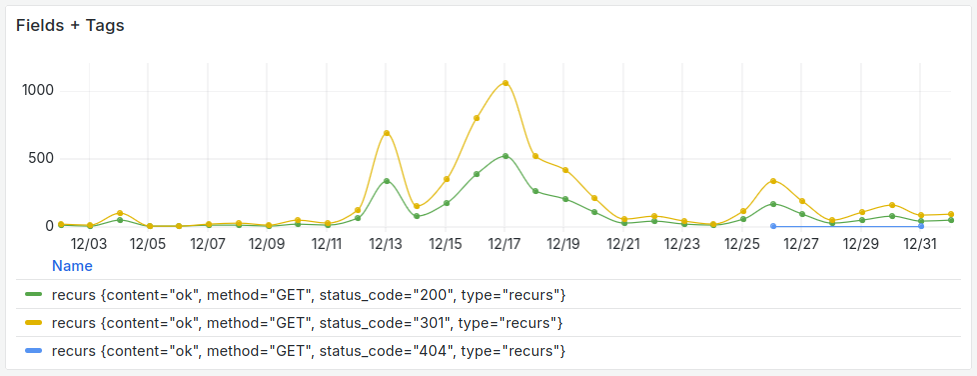
\includegraphics[width=\textwidth]{figures/most-accessed-resource}
        \caption{Recurs més accedit durant el desembre del 2023.}\label{fig:use-case-1}
    \end{figure}
\end{frame}

\begin{frame}{Accessos amb el seu contingut alterat I}
    \begin{itemize}
        \item Donat un espai de temps, volem consultar quants accessos s'han produït amb malformacions al seu contingut.

        \begin{itemize}
            \item Les malformacions del contingut del accessos corresponen a registres que difereixen molt respecte el format general.
            \item Durant l'etapa d'anàlisi i emmagatzematge dels logs, vam marcar aquells sospitosos amb una etiqueta.
        \end{itemize}

        \item També volem esbrinar com ha sigut la seva evolució al llarg del temps, a més dels paràmetres que s'utilitzen.
    \end{itemize}
\end{frame}

\begin{frame}{Accessos amb el seu contingut alterat II}
    \begin{figure}
        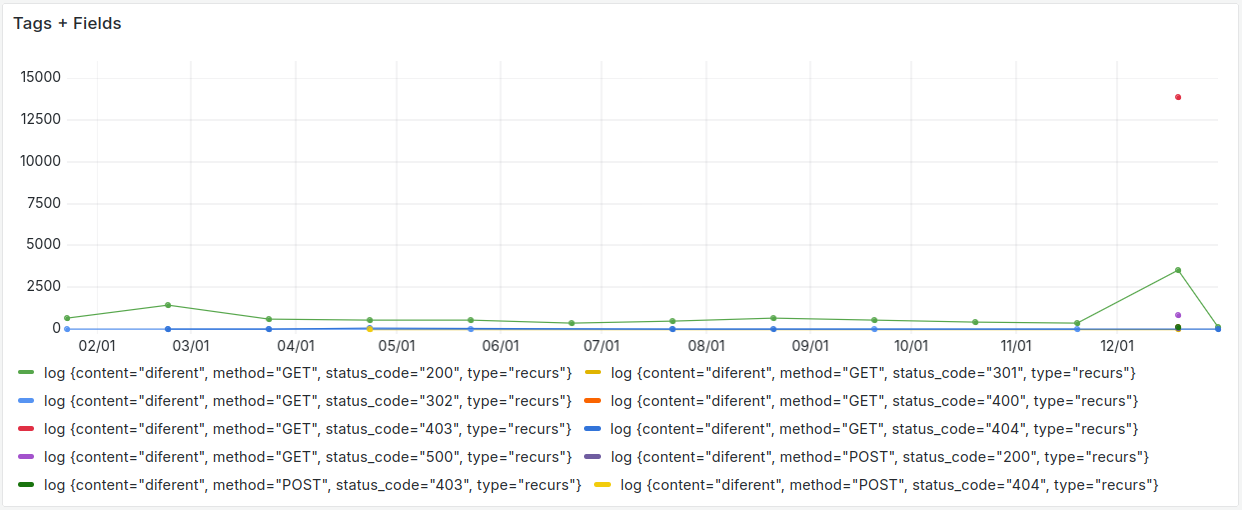
\includegraphics[width=\textwidth]{figures/possible-attacks}
        \caption{Representació dels accessos amb el seu contingut alterat del 2023.}\label{fig:use-case-2}

    \end{figure}
\end{frame}

\begin{frame}{Accessos amb el seu contingut alterat III}
    \begin{figure}
        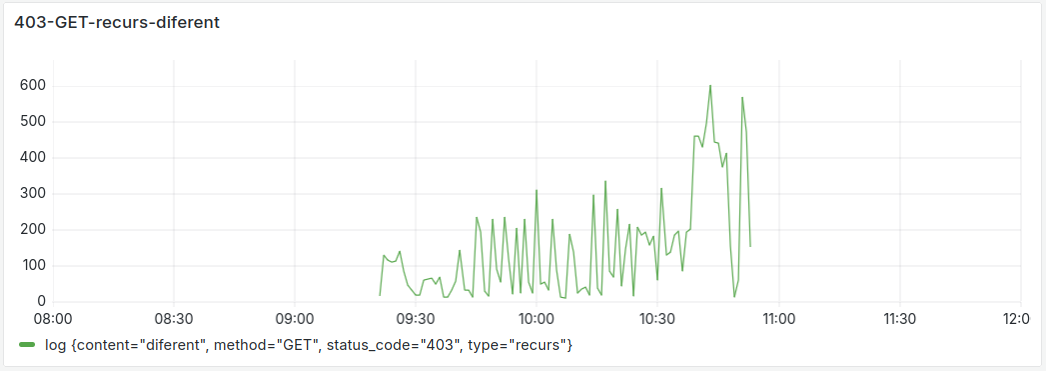
\includegraphics[width=\textwidth]{figures/possible-attacks-403}
        \caption{Pic de peticions del tipus \texttt{GET} que retornen un codi \texttt{403}.}\label{fig:use-case-2-1}
    \end{figure}
    \begin{figure}
        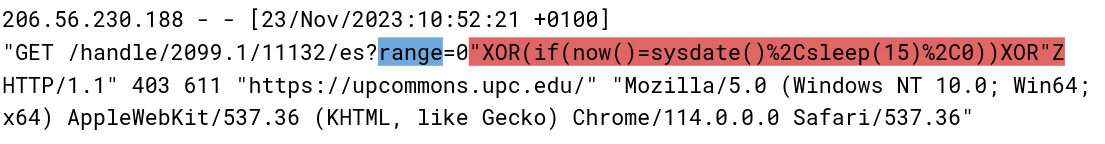
\includegraphics[width=\textwidth]{figures/log-attack}
        \caption{Exemple d'un intent d'atac a través d'un accés a un recurs.}\label{fig:use-case-2-2}
    \end{figure}
\end{frame}

\begin{frame}{Condicions d'accés dels accessos a recursos de l'EPSEVG I}
    \begin{itemize}
        \item Donat un període de temps, volem saber quines són les condicions d'accés dels recursos de l'EPSEVG consultats.
        \item Volem analitzar dels registres aquells que siguin accessos a recursos de l'EPSEVG, i determinar si aquests són d'accés obert, restringits per l'usuari, per acord de confidencialitat, restringit a la comunitat universitària, etcètera.
    \end{itemize}
\end{frame}

\begin{frame}{Condicions d'accés dels accessos a recursos de l'EPSEVG II}
    \begin{figure}
        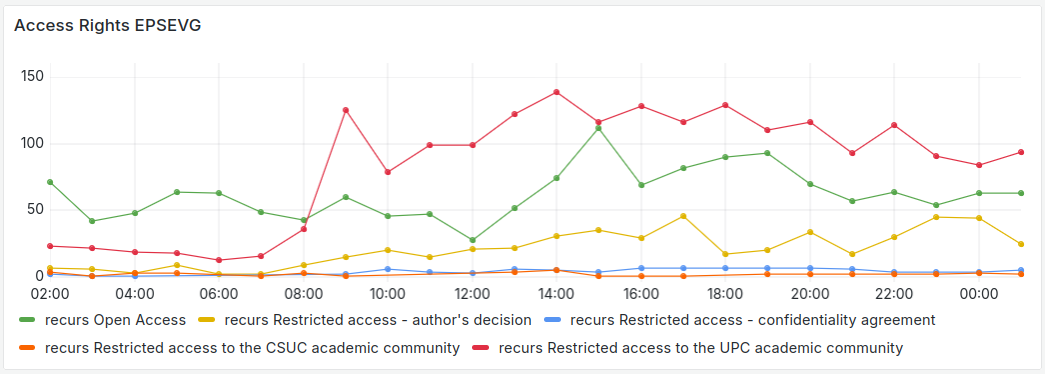
\includegraphics[width=\textwidth]{figures/access-rights-epsevg}
        \caption{Condicions d'accés dels accessos a recursos de l'EPSEVG el primer de desembre del 2023.}\label{fig:use-case-3}
    \end{figure}
\end{frame}
\section{Demostració de l'eina}\label{sec:demo}

\begin{frame}{Demostració}

\begin{itemize}
    \item Repositori de codi de l'eina:
    \begin{itemize}
        \item Open Science Toolkit Information Access.
    \end{itemize}
    \item Servidor de treball:
    \begin{itemize}
        \item Logs i metadades en local.
        \item Bases de dades: MongoDB i InfluxDB.
    \end{itemize}
    \item Grafana:
    \begin{itemize}
        \item Casos d'ús previament presentats.
        \item Presentació de l'estudi d'un cas d'ús nou.
    \end{itemize}
\end{itemize}

\end{frame}


\end{document}